\documentclass{beamer}
\usetheme{Dresden}
%\usetheme{CambridgeUS}
\usepackage{helvet}
\usepackage{cite}
\usepackage{url}
\usepackage{amssymb, amsmath, graphicx, charter, latexsym}
\usepackage{subfigure}
\usepackage{enumerate}
\usepackage{ragged2e}
\usepackage{mathtools}
\usepackage{tabu}
\usepackage{epstopdf}
\usepackage{siunitx}
\usepackage{calligra}
\renewcommand{\familydefault}{\sfdefault}
%\usepackage{times}
\setbeamertemplate{items}[circle]
\setbeamertemplate{navigation symbols}{}
\begin{document}
\title{S-WiFi: Smart Scheduling for WiFi Uplink Transmissions with Point Coordination Function}
\author{Dongni Han, Ping-Chun Hsieh, and Tao Zhao}
\date{April 28, 2016}
\newtheorem{thm}{Theorem}
\begin{frame}
\titlepage
\end{frame}


%\begin{frame}
%\frametitle{What to Discuss Today?}
%\tableofcontents[]
%\end{frame}

%\AtBeginSection[]
%{
	%\begin{frame}{Table of Contents}
	%\tableofcontents[currentsection]
	%\end{frame}
%}

\NewDocumentCommand{\varSI}{O{}}{\SI[detect-all=true,parse-numbers=false,#1]}

\section{Background}

\begin{frame}
\frametitle{System Model}
\begin{itemize}
  \item WiFi network
    \begin{itemize}
      \item One AP and $N$ clients
      % \varSI must be outside math env for it to have right font family.
      \item $\SI{1}{slot} = \SI{10}{ms}$; $\SI{1}{interval} =$ \varSI{T}{slots}
    \end{itemize}
  \item Uplink Transmissions
    \begin{itemize}
      \item Packets generated at each client $n$ in each interval $k$
      \item Number of packets $a_n(k)$ follows Unif$\{U_\text{min}, U_\text{max}\}$
      \item Real-time traffic
    \end{itemize}
  \item Point Coordination Function (PCF)
    \begin{itemize}
      \item AP polls (at most) one client per slot
      \item But AP needs to know $a_n(k)$ first!
    \end{itemize}
\end{itemize}
\end{frame}

\begin{frame}
\frametitle{Baseline Policy: Phase 1}
\begin{itemize}
\item AP polls $a_n(k)$ for all $n$ one by one
\end{itemize}
\begin{figure}
\centering
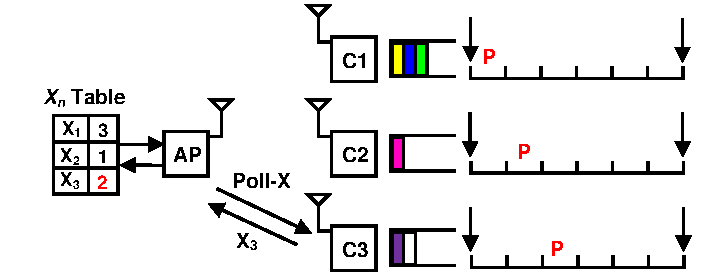
\includegraphics[scale=0.8]{animation_03.pdf}
\end{figure}
\end{frame}

\begin{frame}
\frametitle{Baseline Policy: Phase 2}
\begin{itemize}
\item AP uses Max-Weight scheduling for data transmissions
\end{itemize}
\begin{figure}
\centering
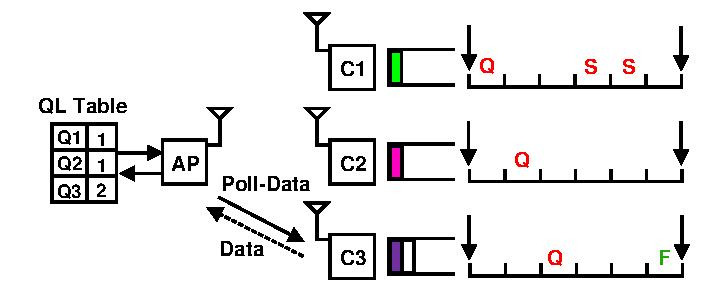
\includegraphics[scale=0.8]{animation_06.pdf}
\end{figure}
\end{frame}

\begin{frame}{Baseline Policy: Issues}
  \begin{itemize}
    \item No data transmissions in Phase 1
    \item Channel utilization for data packets is low
    \item Huge overhead especially with large $N$ and bad channels
    \item We need a smart policy!
  \end{itemize}
\end{frame}
\section{Smart Policy}

\begin{frame}
\frametitle{Idea 1: Selective Polling}
\begin{itemize}
\item Only poll $n \le N$ clients per interval
\item Random permutation for fairness and stability
\item Schedule remaining clients only after all selected are scheduled
\end{itemize}
\begin{figure}
\centering
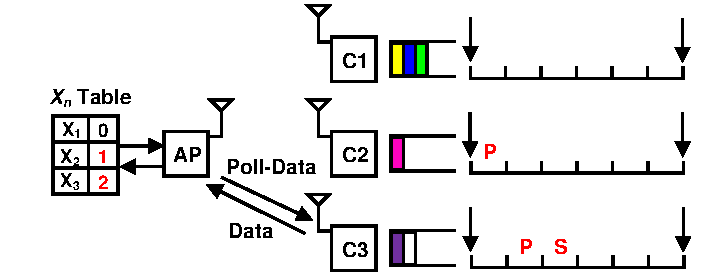
\includegraphics[scale=0.8]{selective_1.pdf}
\caption{Example: $n=2, N=3$}
\end{figure}
\end{frame}


\begin{frame}
\frametitle{Feature 001: Selective Polling}
\begin{itemize}
\item How to determine the optimal $n$?
  \begin{itemize}
    \item Sort clients by channel reliabilities $p_1 > p_2 > \dots > p_N$
    \item Estimated throughput: $\hat{R}_n = \min\{n, (T-\sum_{i=1}^{n}\frac{1}{p_i})\frac{\sum_{i=1}^{n}p_i}{n} \}$
      %fixme
    %\item Find the optimizer $n = \argmax \hat{R}_n$
  \end{itemize}
\item Random permutation?
  \begin{itemize}
    \item Classic problem: random poker shuffling (Knuth)
  \end{itemize}
\item How to schedule remaining clients?
  \begin{itemize}
    \item Greedy: poll $a_n(k)$ and data one by one
  \end{itemize}
\end{itemize}
\end{frame}

\begin{frame}
\frametitle{Idea 2: Piggybacked Queue Length}
\begin{itemize}
\item Queue length can be appended in DATA packets
\end{itemize}
\begin{figure}
\centering
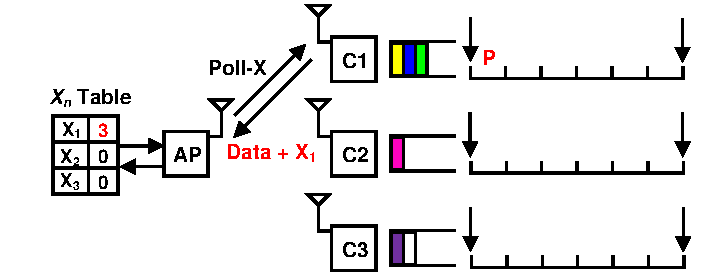
\includegraphics[scale=0.8]{piggyback_1.pdf}
\end{figure}
\end{frame}

\begin{frame}
\frametitle{NS-2 Implementation: Piggybacking}
\end{frame}

\begin{frame}
\frametitle{Idea 3: Retry Limit for Polling}
\begin{itemize}
\item Retry limit: avoid polling a client with poor channel indefinitely
\item Example: $p_1=0.1$ and retry limit = 1
\end{itemize}
\begin{figure}
\centering
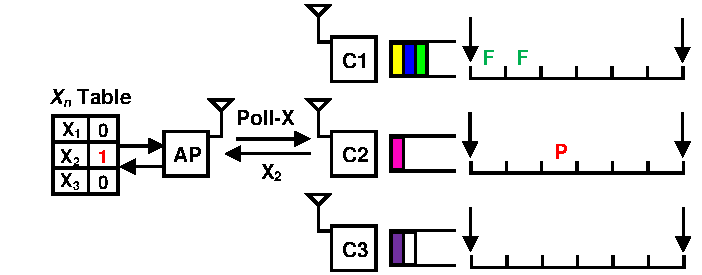
\includegraphics[scale=0.8]{retry_1.pdf}
\end{figure}
\end{frame}

\begin{frame}
\frametitle{NS-2 Implementation: Retry Limit}
\end{frame}

\section{Simulation}
%\begin{frame}
%\frametitle{Simulation Results: Network Capacity}
%\begin{itemize}
%\item $N=2$ and $T=10$
%\item Reliable channel: $p_1 = p_2 = 1$ (symmetric)
%\item $N_\text{max}$ ranges from $1$ to $20$
%\item Real-time traffic
%\end{itemize}
%\begin{figure}
%\centering
%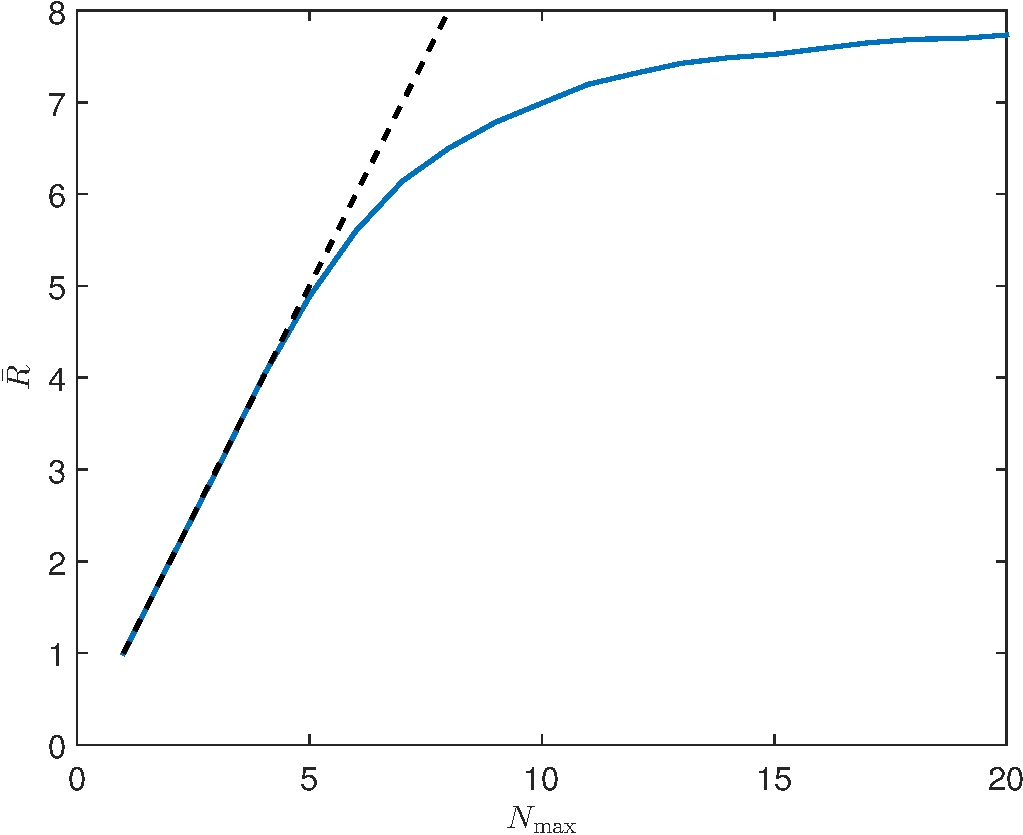
\includegraphics[height=.5\textheight]{realtime_throughput_randmax.pdf}
%\caption{Packet deadline reduces the capacity further.}
%\end{figure}
%\end{frame}

\begin{frame}
\frametitle{Simulation Results}
\begin{itemize}
  \item Fix $T=10$
\item Unreliable channel: $p_1 = p_2 \approx 0.57$ (distance \SI{1000}{m})
\item $N$ ranges from $1$ to $5$
\item Real-time traffic
\end{itemize}
\begin{figure}[htbp]
  \centering
  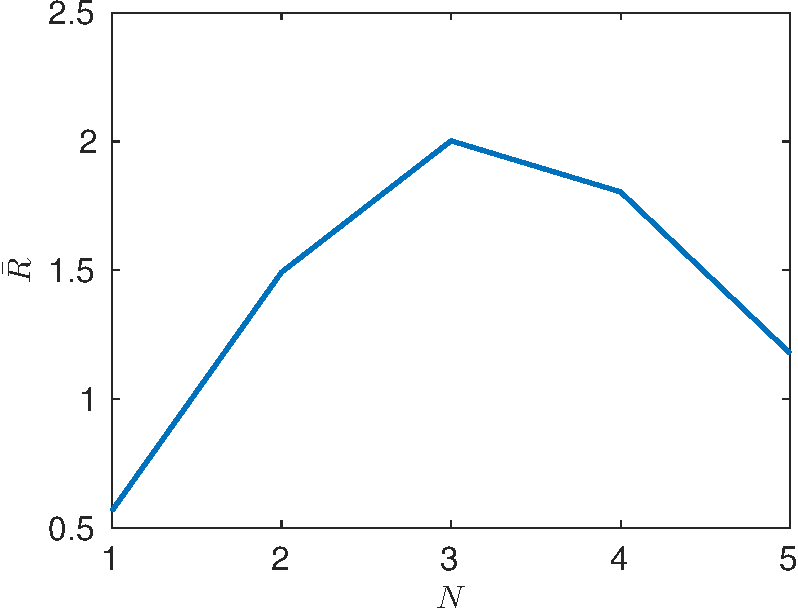
\includegraphics[draft,height=.5\textheight]{realtime_throughput_N.pdf}
  \caption{This is a placeholder!}
\end{figure}
\end{frame}

\section*{Conclusion}
\begin{frame}{Conclusion}
  \begin{itemize}
    \item The baseline policy incurs huge overhead especially with large $N$ and bad channel.
    \item Our smart policy incoporates three major features to improve the performance.
    \item Simulation shows our smart policy can provide up to FIXME times throughput than the baseline policy.
  \end{itemize}
\end{frame}

\begin{frame}
  \begin{center}
    {\Huge\calligra Thank you!}
  \end{center}
  \begin{figure}[htbp]
    \centering
    %FIXME not shown
    
\includegraphics[height=.2\textheight]{url.pdf}
  \end{figure}
\end{frame}
\end{document}
